% !TEX root = ../main.tex

\chapter{Related Work}
\label{chapter:RelWork}
There are three aspects relevant to this thesis:
\begin{itemize}
    \item Imitation Learning
    \item Fine Tuning from Sparse Rewards
    \item Learning in POMDPs with a Single Observation
\end{itemize}
. While to the knowledge of the author, there is no approach specifically tailored for all of these aspects, in this chapter we will cover approaches that involve parts 
of the mentioned aspects and can be used with some limitations in our problem setting.

\section{Single Observation Imitation Learning in POMDPs}
The paper "Language-Conditioned Imitation Learning for Robot Manipulation Tasks" \cite{Language-Conditioned Imitation} proposes a method for robot manipulation tasks that takes 
into account natural language instructions. The proposed method involves using a neural network to map natural language instructions to 
corresponding robot actions. The authors also introduce a novel dataset of language-conditioned robot manipulation tasks, which they use to evaluate 
their method. The experimental results demonstrate the effectiveness of their approach in inferring and executing trajectories for robot manipulation 
tasks when language instructions are given.\\

A policy $\pi(v,I)$ is learned to imitate expert behavior in a set of demonstrations $D = \{d_0,...,d_m\}$, each containing a trajectory 
$R \in R^{T \times N}$ over $T$ time steps and with $N$ control variables, an rgb image $I \in \mathcal{R}^{569 \times 320 \times 3}$ of the agent's surroundings, 
and a task description $v \in \mathcal{R}^{15 \times 50}$ from natural language using GloVe \cite{GloVe} embeddings. The proposed method takes the image $I$ and task description $v$ 
to create a task embedding $e$ using GloVe embeddings and a pretrained image recognition model in the semantic model, 
which is subsequently used in the control model to generate robot actions at each time in a closed-loop 
fashion. A schematic overview can be seen in figure \ref{language_imitation}.

Crucially, there is only one observation per trajectory, so we have a POMDP, where we only know the state of the system at time point $t=0$. In this paper, the 
algorithm uses a GRU to ceep track of the former history of the POMDP, similar to the approach described in \ref{POMDP_RNN}. In addition to the hidden state, 
the task embedding $e$ is used in every timestep, as we know, that the task does not change. \\

\begin{figure}[htbp]
    \centering
    \includegraphics[width=\textwidth]{images/Language_Conditioned/System.pdf}
    \caption{Overview of the general system architecture. (Left) Details of the controller model, which
    synthesizes robot control signals . (Right) details of the semantic model, which extracts critical
    information about the task from both perceptual input and language commands. Dark-blue boxes
    indicate pre-trained components of the model \cite{Language-Conditioned Imitation}.}
    \label{language_imitation}
\end{figure}

The learned behaviour consists of picking up objects and pouring their content into other objects. First, a sentense in natural language describes the object, which 
the agent should pick up. For example "Pick up the red cup". This command in combination with the rgb image of the scene is used to generate the trajectory to 
pick up the cup. Then an object is described, into which the robot should pour the content. For example "Pour some of it into the blue bowl". An overview over 
all possible objects and the described example can be found in figure \ref{lang_imi_expl}. The dataset consists of 45 000 tasks, where 4000 tasks are used for 
evaluation and 1000 tasks are used for testing. The authors find that their model can perform $98 \%$ of pick tasks, $85 \%$ of pour tasks and $84 \%$ combined 
tasks, which greatly outperforms a baseline using an end to end RNN model with $58\%$ success rate for picking and $0 \%$ success rate for pouring.

\begin{figure}[htbp]
    \centering
    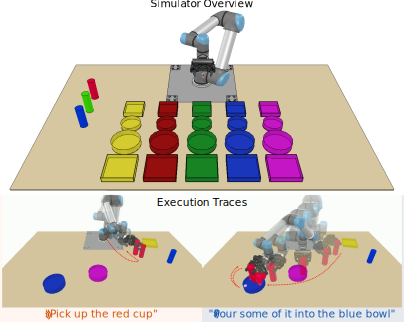
\includegraphics[width=\textwidth]{images/Language_Conditioned/simulator.pdf}
    \caption{Overview of a task. (top) - All possible objects and colors. (left) Example trajectory to "pick up the red cup" following the natural language description. 
    (right) Example trajectory to "pour some of it into the blue bowl". Figure taken from \cite{Language-Conditioned Imitation}.}
    \label{lang_imi_expl}
\end{figure}

\section{Fine Tuning}
Fine-tuning in RL refers to the process of adapting a pre-trained RL model to a new task or environment. In this thesis, fine tuning is done by using behavioural 
cloning on an expert dataset with n trajectories. In the fine tuning phase, the pretrained policy is used in the environment of the task and adiitional feedback 
like sparese rewards are used to enhance the performance of the policy. Fine tuning is a common approach to overcome the exploration problem of high dimensional 
spaces.
\subsection{Sparse Rewards in MDPs with Expert Demonstrations}
In the paper Leveraging Demonstrations for Deep Reinforcement Learning on Robotics Problems with Sparse Rewards \cite{LDDRLP} the authors describe a priority 
sampling algorithm in combination with the deep deterministic policy gradient (DDPG) algorithm as described in \ref{AC-Alg}. The probability with which a 
training sample is chosen from the replay buffer is described as:
\begin{equation}
    P(i) = \frac{p_i^\alpha}{\sum\limits_{k} p_k^\alpha}
\end{equation}
with 
\begin{equation}
    p_i = \delta_{i}^2 + \lambda \lvert \nabla_a Q(s_i, a_i \vert \theta_Q) \rvert^2 + \epsilon + \epsilon_{D}.
\end{equation}
Here $\delta_{i}$ is the temporal difference error, $\lambda$ is used to weigh the importance of the sample i with respect to the loss of the actor, 
$\epsilon$ is a small constant to ensure every transition is chosen with probability $p_i > 0$ and $\epsilon_D$ is a positive constant aplied for expert transitions.\\
The idea behind this importance sampling algorithm is to amment the priority experience replay probability as developed in \cite{https://arxiv.org/pdf/1511.05952.pdf} 
with a constant $\epsilon_{D}$ for expert demonstrations to make the policy converge faster to the expert behaviour. In priority experience replay, more rare 
experiences are chosen more likely to use the data in the replay buffer more efficiently. Moreover, they use a combination between $n=1$ temporal difference and 
$n=N > 1$ temporal difference to get better estimations for rewards that are in the distant future, as they assume sparse rewards.\\
The effectiveness of the approach is demonstrated by comparing the performance of their importance sampling algorithm with sparse rewards to a standard DDPG 
implementation using no expert demonstration but dense reward. The authors find that their approach can learn faster then standard DDPG with 100 expert 
demonstrations on a challenging robotic insertion task.\\ 
A problem with this approach is, that the critic assumes the demporal difference error approximates the distribution induced by the policy $\pi_{\theta}$, but by 
mixing in expert demonstrations, the expected $Q$ value will be higher, then that of the policy $\pi_{\theta}$. This overestimation can lead to poor performance. 
The authors include a term to "weigh the update to the network" $w_i = \frac{1}{N} \cdot \frac{1}{P(i)}$. This term however is inversly proportinal to the 
probability of choosing a transition and thus counter acts the improvement rate towards expert behaviour.
\subsection{GAIL in POMDPs}
Recall that GAIL optimized the objective
\begin{equation*}
    \min_{\theta} \max_{\omega} \mathbb{E}_{(s,a)\sim \pi_{\theta}, \mathcal{T}} [\log(1 - D_{\omega}(s,a))] + \mathbb{E}_{(s,a)\sim \mathcal{M}_{\text{E}}} [\log D_{\omega}(s,a)]
\end{equation*}
as derived in \ref{GAIL_Obj}, where $\mathbb{E}_{(s,a)\sim \mathcal{M}_{\text{E}}}$ denotes the expected distribution of the expert policy and 
$\mathbb{E}_{(s,a)\sim \pi, \mathcal{T}}$ denotes the expected distribution of the learned policy $\pi$, $D_{\omega}$ is the discriminator measuring how likely a state 
action pair was induced by the expert policy or the learned policy $\pi_{\theta}$. The paper "Learning Belief Representations for Imitation Learning in POMDPs" \cite{https://arxiv.org/pdf/1906.09510.pdf} 
extends the GAIL paradigm to work on POMDPs. To do so, they intorduce a network $B_{\phi}(o_{\leqt}, a_{\leqt}) = b_{t, \phi}$ that aims to approximate a 
representation of the beliefe state $b_t$ \ref{pomdp_bayes}, which forms a sufficient statistic for the POMDP 
$p(s_t|o_{\leq t}, a_{\leq t}) = p(s_t|b_t) \approx p(s_t|b_{t, \phi})$. Using $b_{\phi}$ instead of $s$ the new objective is:
\begin{equation}
    \min_{\phi,\theta}\max_{\tilde{\omega}} &\mathbb{E}_{(b,a)\sim\mathcal{M}_{\text{E}}}[\log D_{\tilde{\omega}}(b_{\phi},a)] + \mathbb{E}_{(b,a)\sim\pi,\mathcal{T}}[\log(1-D_{\tilde{\omega}}(b_{\phi},a))]
\end{equation}
. The authors include three regularisation losses to improve the expressiveness of $b_{\phi}$ of the form 
\begin{equation}
    \mathcal{L}^f(\phi) = \mathbb{E}_{\mathcal{R}} ||f_{\text{goal}}(t, k) - g(b_t^\phi, \text{input}_{t, k})||_2^2
\end{equation}, 
where they un